\usetikzlibrary{arrows}

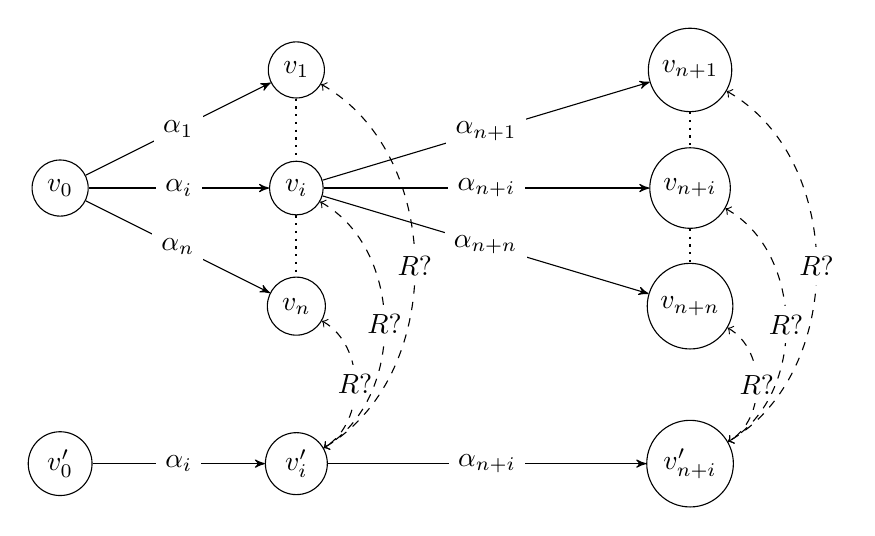
\begin{tikzpicture}[node distance=3cm]
\node[draw,circle] (u0) {$v_0$};
\node[draw,circle, right of = u0] (ui) {$v_i$};
\node[draw,circle, above of = ui,yshift=-1.5cm] (u1) {$v_1$};
\node[draw,circle, below of = ui,yshift=1.5cm] (un) {$v_n$};

\node[draw,circle, right of = ui,xshift=2cm] (uni) {$v_{n+i}$};
\node[draw,circle, above of = uni,yshift=-1.5cm] (un1) {$v_{n+1}$};
\node[draw,circle, below of = uni,yshift=1.5cm] (unn) {$v_{n+n}$};

\node[draw,circle, below of = u0,yshift=-.5cm] (v0) {$v'_0$};
\node[draw,circle, right of = v0] (vi) {$v'_i$};
\node[draw,circle, right of = vi,xshift=2cm] (vni) {$v'_{n+i}$};

\path
(u1) edge[dotted,thick] (ui)
(ui) edge[dotted,thick] (un)
(un1) edge[dotted,thick] (uni)
(uni) edge[dotted,thick] (unn)

(un) edge[<->,dashed,bend left = 60] node[fill=white] {$R$?} (vi)
(ui) edge[<->,dashed,bend left = 60] node[fill=white] {$R$?} (vi)
(u1) edge[<->,dashed,bend left = 60] node[fill=white] {$R$?} (vi)

(unn) edge[<->,dashed,bend left = 60] node[fill=white] {$R$?} (vni)
(uni) edge[<->,dashed,bend left = 60] node[fill=white] {$R$?} (vni)
(un1) edge[<->,dashed,bend left = 60] node[fill=white] {$R$?} (vni)

(u0) edge[->,>=stealth'] node[fill=white] {$\alpha_1$} (u1)
       edge[->,>=stealth'] node[fill=white] {$\alpha_i$} (ui)
       edge[->,>=stealth'] node[fill=white] {$\alpha_n$} (un)
(ui) edge[->,>=stealth'] node[fill=white] {$\alpha_{n+1}$} (un1)
       edge[->,>=stealth'] node[fill=white] {$\alpha_{n+i}$} (uni)
       edge[->,>=stealth'] node[fill=white] {$\alpha_{n+n}$} (unn)
(v0) edge [->,>=stealth'] node[fill=white] {$\alpha_i$} (vi)
(vi) edge [->,>=stealth'] node[fill=white] {$\alpha_{n+i}$} (vni)
;
\end{tikzpicture}
